	\section{Hierarchical Clustering and Principle Component Analysis (PCA)}
	\resetquestioncounter{}
	\begin{qanda}
		\begin{question}
PCA explained how to reduce dimensions on the data set, However, when solved, there is no info on which dimensions (columns) are the most important and which we can remove. How can I know that information?
		\end{question}
		\begin{answer}
Using PCA, the columns are completely changed. PCA finds a new relationship between the columns. So, we use it to get a higher score. If the focus is to find feature importance, then PCA fails as it completely transforms the columns and new columns will not mean the same as the older ones, so we cannot name them. Feature importance after PCA will make no sense at all.

After transforming columns using PCA we try to take the minimum number of columns through which we can achieve the maximum score.
		\end{answer}
	\end{qanda}


	\begin{qanda}
		\begin{question}
How do we choose the correct distance to use in clustering algorithms?
		\end{question}
		\begin{answer}
There is no single distance that will give the best results with all data and all problem statements. The type of distance you use depends on the data and the problem statement. Generally normalized Euclidean distance is used. However, when data size is very large and high dimensional, Manhattan distance is found to perform better computationally. The type of distance to use is decided by the problem at hand.
		\end{answer}
	\end{qanda}


	\begin{qanda}
		\begin{question}
What then do we do with the clusters after interpretations?
		\end{question}
		\begin{answer}
What you do with clusters after interpretation depends upon the problem you are trying to solve. Clustering will give you groups that are similar in some aspects. This can be used for recommendations, understanding customers, market campaigning, etc. Again what you do after interpretation of clustering depends upon what problem you are trying to solve.
		\end{answer}
	\end{qanda}

	\begin{qanda}
		\begin{question}
How do we know whether K-means or hierarchical clustering is appropriate to use in a given business problem?
		\end{question}
		\begin{answer}
The k-means algorithm is used when it is already known in advance how many clusters have to be formed, also k-means is suitable if your data is well separated into spherical-like clusters. On the other hand, hierarchical clustering is density-based clustering in which nearby points are joined to form clusters. It gives you a dendrogram from which you can figure out how many clusters should be formed. Hierarchical clustering is computationally expensive so it will not perform well when the data size is very very big.
		\end{answer}
	\end{qanda}

	\begin{qanda}
		\begin{question}
I get the following error when I try to use SilhouetteVisualizer with AgglomerativeClustering.
AttributeError: `AgglomerativeClustering' object has no attribute `predict'
Why does this throw the error and how to debug this?
		\end{question}
		\begin{answer}
The SilhouetteVisualizer function from yellowbrick library is designed for visualizing the cluster of K-means only as you can read from its documentation. If you want to find the silhouette score for clusters obtained using hierarchical clustering, then you have to use sklearn function of silhouette score which is given here.

A sample code is given below

score = silhouette\_score(X, HCmodel.labels\_, metric=`euclidean')
where X is a scaled dataset, and HCmodel is the agglomerative model fit on the data set.
		\end{answer}
	\end{qanda}

	\begin{qanda}
		\begin{question}
Are correlated features a problem when it comes to clustering? If so can you point me to why this might be a problem?
		\end{question}
		\begin{answer}
First of all, you have to decide which variables you should be used for clustering, Once you have done that, it is better to choose only those variables among them, such that no two variables have a correlation of more than 0.7 (magnitude).

Correlation does not have a negative impact on clustering but removing correlated variables helps to reduce the dimension and can be computationally efficient when you have a very large number of observations.
		\end{answer}
	\end{qanda}

	\begin{qanda}
		\begin{question}
How do we select the optimal number of clusters from the Dendrogram?
		\end{question}
		\begin{answer}
Choosing the optimal number of clusters is a fairly subjective matter, and the best method to identify the optimum number of clusters is to use a combination of metrics and domain expertise. The dendrogram is one of the most common ways for estimating the appropriate number of clusters for hierarchical clustering if we don't have domain expertise.

The optimal number of clusters from a dendrogram can be obtained by deciding where to cut the cluster tree. Generally, the cluster tree is cut where the dendrogram height is maximum as it corresponds to distinct and homogeneous clusters.

Please refer to the \figurename~\ref{fig:hierarchicalclustering} for an example, the distance between the red horizontal lines denotes the maximum distance that has been traversed without intersecting any cluster. So, the ideal number of clusters, from the above dendrogram can be 4 clusters. However, one should also do cluster profiling and check if the cluster profiles are meaningful and have variability, for which domain knowledge is needed.

We can get a different number of clusters from the dendrogram at different heights. But the standard approach to picking the appropriate number of clusters from the dendrogram is to check the maximum height of the vertical line formed.
		\end{answer}
	\end{qanda}

	\begin{figure}[h]
		\centering
		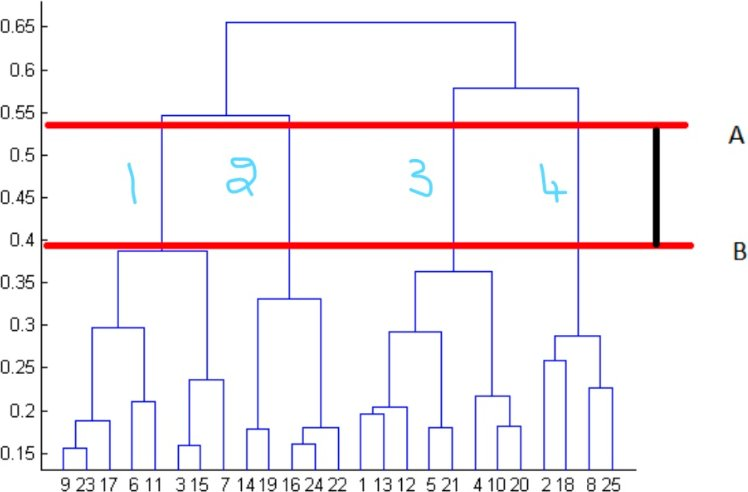
\includegraphics[height=2.0in]{hierarchicalclustering}
		\caption{Hierarchical clustering.}
		\label{fig:hierarchicalclustering}
	\end{figure}

	\section{Top Down or Bottom Up}
In the divisive or top-down clustering method we assign all of the observations to a single cluster and then partition the cluster into two least similar clusters.

In the agglomerative or bottom-up clustering method we assign each observation to its cluster. Then, compute the similarity (e.g., distance) between each of the clusters and join the two most similar clusters.

	\section{Dimensionality Reduction}
	\begin{bulletedlist}
		\item The process of reducing the number of independent variables.
		\item Reducing dimensionality of independent variables helps in many ways.
		\begin{bulletedlist}
			\item Removes multi-collinearity to improve machine learning model performance.
			\item Helps reduce over fitting.
			\item Decreases computational times for fitting models.
			\item Make visualization easier.
			\item Decreases storage requirements.
			\item Avoids curse of dimensionality.
		\end{bulletedlist}
		\item Dimensionality reduction plays a significant role in analyzing data.
	\end{bulletedlist}

	\section{Dimensionality Reduction Techniques}

	\begin{bulletedlist}
		\item Feature elimination.
		\begin{bulletedlist}
			\item Simply identify and remove variables (columns) that are not important.
			\item The disadvantage is that we would gain no insight from those dropped variables and loose any information they contain.
		\end{bulletedlist}
		\item Feature action.
		\begin{bulletedlist}
			\item Create a few new variables from the old variables
			\item PCA  Principal Component Analysis: is the most popular feature extraction technique (linear)
			\item t-SNE (non-linear)
		\end{bulletedlist}
	\end{bulletedlist}

	\section{Principle Component Analysis (PCA)}
	\begin{bulletedlist}
		\item Creates new variables using linear combinations of old variables.
		\item Is designed to create variables that are independent of one another.
		\item Also manages to tell us how important each of these new variables are.
		\item This ``importance,'' helps us to choose how many variables we will use.
		\item Scale the data and compute the covariance matrix.
		\item Break the covariance matrix into magnitude and direction. Eigenvectors and the Eigenvalues of the covariance matrix can be thought of as the natural axis/directions and magnitudes along those axis, of the data.
		\begin{bulletedlist}
			\item The eigenvalues also can be used to calculate the percentage of variation explained by each component.
		\end{bulletedlist}
		\item Soft in the eigenvalues in descending order and calculate the cumulative percentage of variation explained.
		\item Pick the number of principal components you will use.
		\item Transform to new variables.
	\end{bulletedlist}

	\begin{figure}[h]
		\centering
		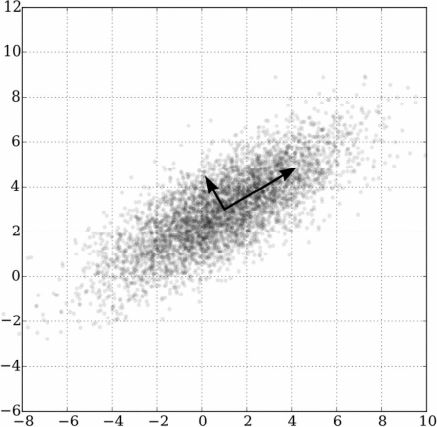
\includegraphics[height=2.0in]{principalcomponentanalyis}
		\caption{.}
		\label{fig:principalcomponentanalyis}
	\end{figure}
 	\begin{figure}[h]
		\centering
		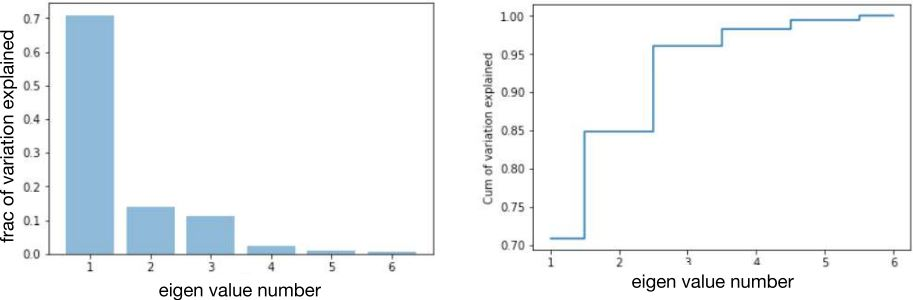
\includegraphics[height=2.0in]{eigenvaluesandvariation}
		\caption{.}
		\label{fig:eigenvaluesandvariation}
	\end{figure}

	\section{Cophenetic Correlation}
Used to compare different clustering results.

Takes a measurement type and calculates all the distances between the points and the heights in the dendrogram that they combine at.  If the correlation of these two columns is a measure of how good the dendrogram is.

	\section{t-SNE}
t-distributed stochastic neighbor embedding a non-linear technique for combining features.  It is only used for visualization.
	\begin{bulletedlist}
		\item A non-linear dimensionality reduction technique which is mainly used for visualization purposes of high dimensional data.
		\item Maps high-dimensional data to 2 or 3 dimensions, making it easier for us to visualize.
		\item Tries to preserve local structure in the data.
		\begin{bulletedlist}
			\item This is done by preserving the distribution of the data found in higher dimension to the lower dimension as much as possible.
			\item This means that points that are closer to each other in the higher dimension are close in the lower dimension too, and the points far apart from each other in the higher dimension are far apart in the lower dimension too.
		\end{bulletedlist}
	\end{bulletedlist}

	\subsection{How Does it Work}
	\begin{bulletedlist}
		\item Compute a distribution that measures pairwise similarities in original data (high dimensional space).
		\item Find a ``close'' lower dimensional distribution of pairwise similarities.
		\item Use this mapping to transform higher dimensional data into lower dimensional data.
		\item Finding this ``close''  technically involves minimizing the divergence between two distributions.  The minimization is usually achieved using stochastic gradient descent and Kullback-Leibler divergence is usually the measure of divergence.
	\end{bulletedlist}

 	\begin{figure}[h]
		\centering
		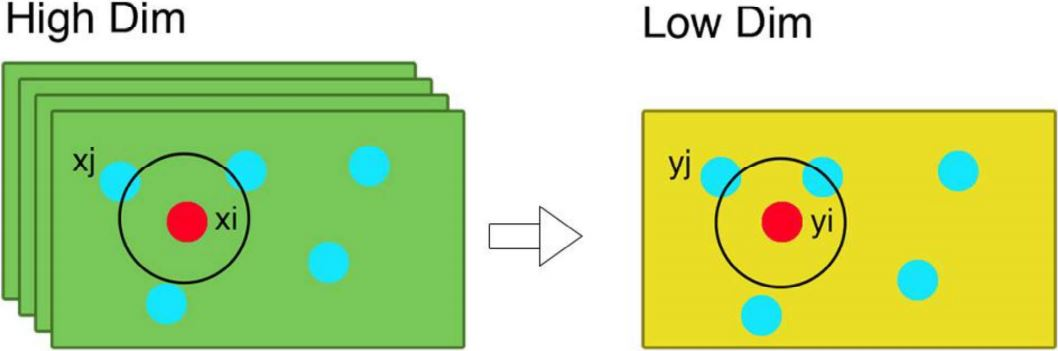
\includegraphics[height=1.0in]{tsnedimensionalreduction}
		\caption{.}
		\label{fig:tsnedimensionalreduction}
	\end{figure}

	\subsection{Steps Involved in t-SNE}
	\begin{bulletedlist}
		\item Scale the data.
		\item Compute the similarity of data points in high dimensional space.
		\item Compute the similarity of data points in the corresponding lower dimensional space.
		\item Minimize the distance between these two distributions using KL divergences.
		\item The lower dimensional distribution obtained when the algorithm converges is the lower dimensional representation of the original data.
	\end{bulletedlist}

	\subsection{Choosing the Right Perplexity}
	\begin{bulletedlist}
		\item We find patterns by identifying observed clusters based on similarity of data points with multiple features.  However, after this process, the input features are no longer identifiable. and you cannot make any inference based only on the output of t-SNE.  Hence it is mainly a data exploration and visualization technique.
		\item The hyperparameter ``perplexity'' in some sense captures the balancing act between local and global aspects of the data.  It has a significant effect on the resulting visualization.
		\item Perplexity can also be thought of as the guess on the number of neighbors.
		\item The range of values recommended for perplexity is between 5 and 50.
	\end{bulletedlist}

 	\begin{figure}[h]
		\centering
		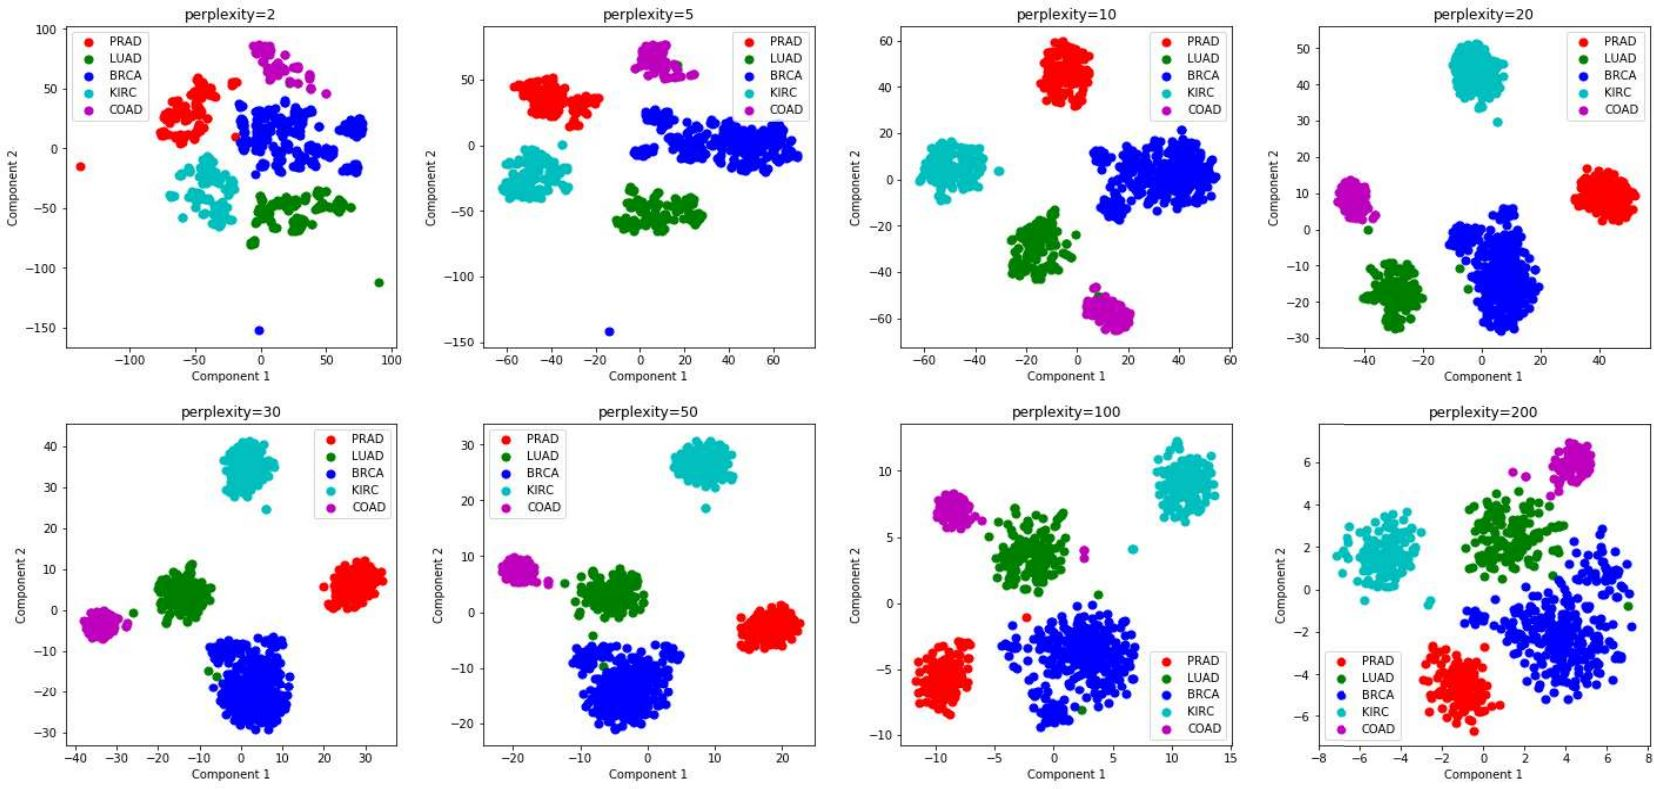
\includegraphics[width=\textwidth]{perplexityvaluesfortsne}
		\caption{.}
		\label{fig:perplexityvaluesfortsne}
	\end{figure}

	\subsection{PCA versus t-SNE}
	\begin{tabular}{|p{0.5\textwidth-2\tabcolsep}|p{0.5\textwidth-2\tabcolsep}|} \hline
			\tablecolumnheadervlinesone{PCA} & \tablecolumnheadervlinestwo{t-SNE} \\ \hline
			Linear &
            Non-linear \\ \hline
			Maximizes the variance capture to find the structure within the data. &
			Relies on probability distributions to find the structure within the data.  \\ \hline
			Seeks to preserve all pairwise distances. &
			Seeks to preserve small pairwise distances. \\ \hline
			Tries to preserve global structure only. &
			Tries to preserve local structure only. \\ \hline
			Computational time is low. &
			Computational time is high. \\ \hline%
		\end{tabular}


	\subsection{Why use t-SNE Over PCA for Visualization}
	\begin{bulletedlist}
		\item The visualization illustrates how distances between points are computed by PCA (dotted line) and t-SNE (solid line).
		\item The points, which are actually distant as per structure of data, are interpreted as similar (close) by PCA.
		\item However, t-SNE captures the local structure correctly and interprets them as dissimilar (far apart).
	\end{bulletedlist}

 	\begin{figure}[h]
		\centering
		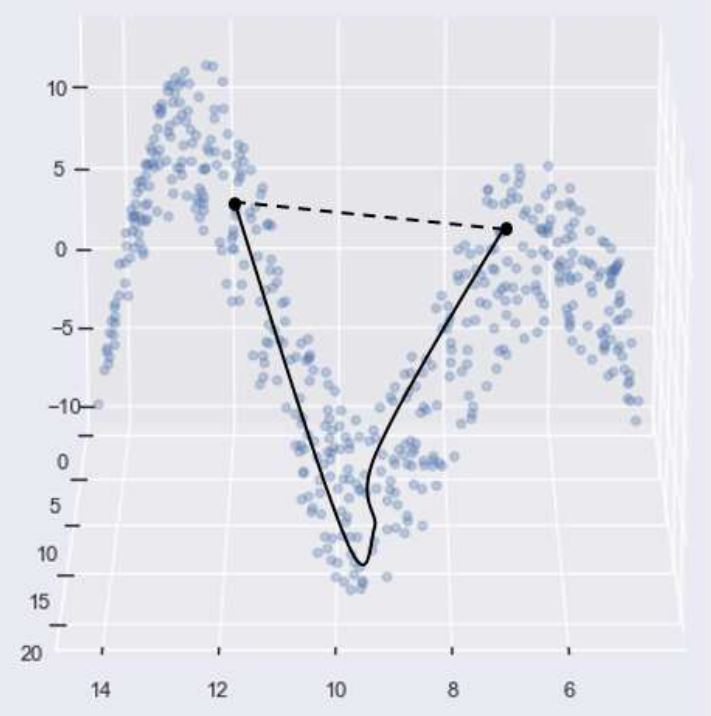
\includegraphics[height=2.25in]{tsneversuspca}
		\caption{.}
		\label{fig:tsneversuspca}
	\end{figure}

